% ----------------------------------------
% LaTeX Article Template for CUED Reports by Jon Sowman, 2009 (jon@hexoc.com)
% ----------------------------------------

\documentclass[12pt]{article} % Set up the document class for an article
\usepackage[margin=2.5cm]{geometry}
%\usepackage{savetrees}		% Concise layout
\usepackage{amssymb}		% This packages permits using $ \therefore $
\usepackage{graphicx}		% SVG graphics includes, amongst other things
\usepackage{epstopdf}		% Allows EPS graphics includes
\usepackage{amsmath}		% This package allows the use of $ \text{} $
\usepackage{placeins}		% This package allows the use of \FloatBarrier
\usepackage{caption}		% This package allows subfigures:
\usepackage{subcaption}	    % And proper subfigure captioning
\usepackage{appendix}
\usepackage[amssymb]{SIunits}
\usepackage{xspace}
\usepackage{bold-extra}
\usepackage{tikz}

\usetikzlibrary{decorations.pathreplacing}
\usetikzlibrary{patterns}
\usetikzlibrary{calc}

\newcommand{\thegrid}{\textsc{the\textperiodcentered grid}\xspace}
\newcommand{\amaze}{\textsc{aMAZE}\xspace}

\title{\thegrid\\\small{\textsc{Interactive Display Matrix}}}
%\title {\textsc{emission}\\\large{\textsc{The Grid}}}
\author{\small{David Turner (dwt27@cl.cam.ac.uk)}\\
        \small{Adam Greig (ag611@eng.cam.ac.uk)}}
\date{} %Suppress date

% Begin the document
\begin{document}
\maketitle

\renewcommand{\abstractname}{Summary}
%%%%%%%%%%%%%%%%%%%%%%%%%%%%%%%%%%%%%%%%%%%%%%%%%%%%%%%%%%%%%%%%%%%%%%%%%%%
\begin{abstract}
\thegrid is an art/engineering installation consisting a grid of poles
illuminated by white LED strips.  Interactivity is provided through a computer
vision system utilising a night vision camera.  Applications include a virtual
maze and interactive display patterns.  Primary requirements are a $14\metre
\times 18\metre$ area of unlit ground and access to mains power (approx
$1.5\kilo\watt$ peak).
\end{abstract}

\begin{figure}[h]
    \centering
    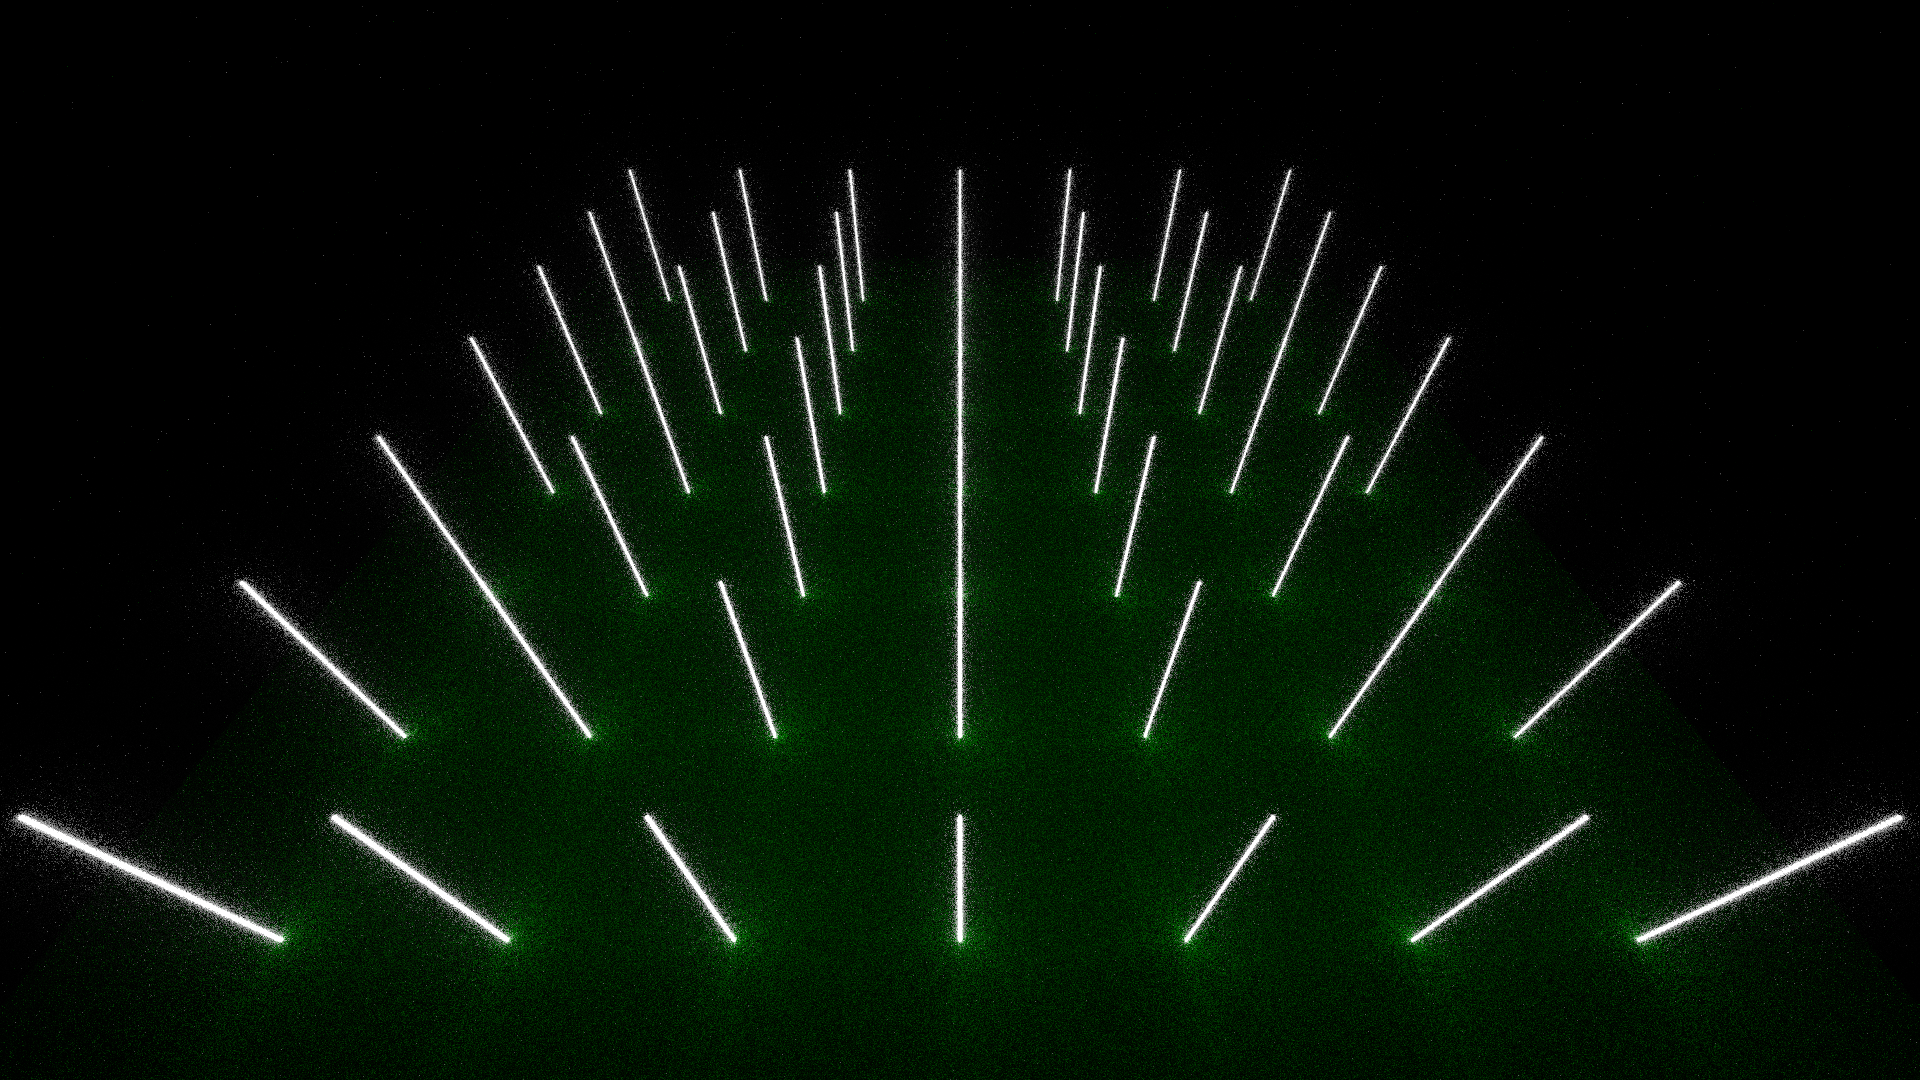
\includegraphics[width=\textwidth]{pics/render1.png}
    \caption{A computer graphics simulation of \thegrid.}
\end{figure}

%%%%%%%%%%%%%%%%%%%%%%%%%%%%%%%%%%%%%%%%%%%%%%%%%%%%%%%%%%%%%%%%%%%%%%%%%%%
\clearpage
\section{Design}
\subsection{Layout}
\thegrid would occupy a space of approximately $18\metre \times 14\metre$.  Of
this, $12\metre \times 12\metre$ is the grid itself, consisting of a $7 \times
7$ grid of poles with $2\metre$ spacing.  A backstage area holds the power and
control tent as well as the camera mast.

\begin{figure}[h]
    \centering
    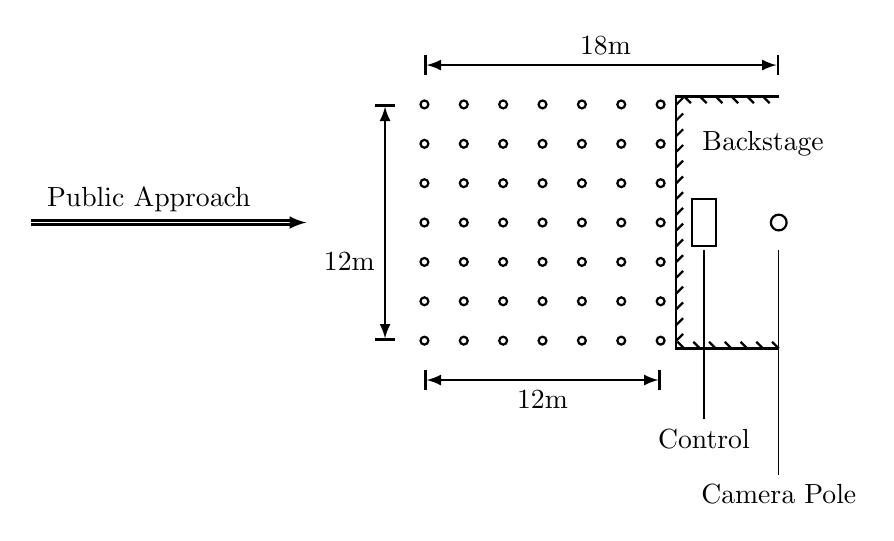
\begin{tikzpicture}[
        >=latex, thick,
    ]
    \foreach \x in {0.0cm, 0.5cm, 1.0cm, 1.5cm, 2.0cm, 2.5cm, 3.0cm}
        \foreach \y in {-1.5cm, -1.0cm, -0.5cm, 0.0cm, 0.5cm, 1.0cm, 1.5cm}
            \draw (\x, \y) circle (0.5mm) coordinate (\x\y);

    \draw (4.5cm, -1.6cm) -- (3.2cm, -1.6cm) -- (3.2cm, 1.6cm) -- (4.5cm, 1.6cm);
    \draw[decoration={border,segment length=2mm,amplitude=1.2mm,
                      mirror,angle=45},decorate]
         (4.5cm, -1.6cm) -- (3.2cm, -1.6cm) -- (3.2cm, 1.6cm) -- (4.5cm, 1.6cm);
    \draw (3.4cm, 1.0cm) node[right] {Backstage};

    \draw (3.4cm, -0.3cm) rectangle (3.7cm, 0.3cm) coordinate (control);
    \draw[thin] (3.55cm, -0.35cm) -- (3.55cm, -2.5cm) node[below] {Control};

    \draw (4.5cm, 0.0cm) circle (1mm) coordinate (camera);
    \draw[thin] (4.5cm, -0.35cm) -- (4.5cm, -3.2cm) node[below] {Camera Pole};

    \draw[->, double] (-5.0cm, 0.0cm) -- (-1.5cm, 0.0cm);
    \draw (-3.5cm, 0.0cm) node[above] {Public Approach};

    \draw[|<->|] (0cm, -2.0cm) -- (3.0cm, -2.0cm);
    \draw (1.5cm, -2.0cm) node[below] {12m};

    \draw[|<->|] (-0.5cm, -1.5cm) -- (-0.5cm, 1.5cm);
    \draw (-0.5cm, -0.5cm) node[left] {12m};

    \draw[|<->|] (0cm, 2.0cm) -- (4.5cm, 2.0cm);
    \draw (2.3cm, 2.0cm) node[above] {18m};

    \end{tikzpicture}
    \caption{Plan schematic}
    \label{fig:planschematic}
\end{figure}

\subsection{Structural}
Each pole will protrude $2.5\metre$ from the ground.  The total length is
$3\metre$, with $50\centi\metre$ being inserted into the ground.  The poles are
constructed from $\frac{3}{4}" \times \frac{3}{4}" \times \frac{1}{16}"$
aluminium angle section.  See Appendix~\ref{app:engdrawings} for detailed
drawings.

The interactivity camera will be mounted $8\metre$ above the ground on a
$10\metre$ fishing pole, guyed for rigidity.

\subsection{Electrical and Electronics}
\subsubsection{Cabling}
Each LED strip will consume around $2\ampere$ when active.  The wiring for one
strip will consist of twin core cable carrying power and return between the
strip and the control tent.  Additionally, a coaxial connection will run from
the interactivity camera to the control tent.

Ideally, all cabling inside \thegrid will be buried slightly below ground to
avoid a trip hazard.  If this is not possible, cabling could be run between the
tops of poles at a height of $2.5\metre$.

\subsubsection{Switching}
Each LED strip will be controlled using a BD679
Darlington pair as a driver.  The drivers will be switched by six 8-output
shift registers, themselves controlled by the CPU.

\subsubsection{Power}
The maximum power consumption of \thegrid will be
$100\ampere$.  This will be provided by four $550\watt$ ATX power supplies,
each rated for $32\ampere$ on its $+12\volt$ rail.

\subsection{Software and Control}
A laptop in the control tent will generate
display patterns and handle interactivity.  It will transmit lighting data via
a serial link to an Arduino.  Upon receiving each frame, the Arduino will clock
the data into the shift registers, then activate the output latch.

A night vision enabled camera (with separate IR floodlight) mounted on a mast
in the backstage area senses movement and tracks the location of people inside
\thegrid.  This information is used for interactive applications and patterns.

%%%%%%%%%%%%%%%%%%%%%%%%%%%%%%%%%%%%%%%%%%%%%%%%%%%%%%%%%%%%%%%%%%%%%%%%%%%
\section{Applications}
\subsection{\amaze}
\amaze is an interactive, virtual maze.  In this mode, when a user enters
\thegrid, a maze is randomly generated.  Squares the user can travel to are
lit, while squares representing walls are dark.  \amaze monitors the user's
progress and knows if the user completes the maze, or cheats!  The twist is
that \amaze only lights the user's square and adjacent squares---the user
cannot see ahead and can only explore passages by travelling them!

A variation on this is two-player \amaze.  Two players can simultaneously
traverse different (and overlapping) mazes, competing for time.

\subsection{Interactive Patterns}
A number of interactive patterns will produce interesting visual effects based
on the movement of people in \thegrid, inspired by fluid disturbance and flow.

\subsection{Non-interactive Patterns}
For times when no users are directly interacting with \thegrid, non-interactive
patterns will display pre-programmed effects resembling waves, stars and
sparks.

%%%%%%%%%%%%%%%%%%%%%%%%%%%%%%%%%%%%%%%%%%%%%%%%%%%%%%%%%%%%%%%%%%%%%%%%%%%
\clearpage
\section{Risk Assessment}
\subsection{Mechanical}
\thegrid is an interactive exhibit designed for people to walk around.  It is
also active after sunset.  This leads to a number of risks due to people
walking around and through a structure in low lighting.  However, it is
anticipated that there is a minimal risk of injury.  As poles are embedded in
soft ground and are constructed from thin aluminium section, it is anticipated
that there is no serious risk of injury should somebody walk into a pole.

Poles will be $2.5\metre$ (8 foot 2 inches) tall, so there should be no risk of
impalement or eye injury.

In the very unlikely case of a pole falling on a person, the pole's light
weight (around $500\gram$) should mean there is minimal possibility for injury.

With people walking around the installation in low light, there would be a
significant trip hazard were any cabling or guy-wires exposed.  For this
reason, all cabling inside \thegrid itself will be buried below the surface of
the ground.  If the cable cannot be buried, it could be run overhead between
the top of the poles.  Again, this is high enough that it should be impossible
to walk into.

The backstage area will contain cabling running at ground level alongside other
hazards, and so will be off limits.

\subsection{Electrical}
All mains electronics will be contained within the control tent and power is
distributed through \thegrid at $12\volt$ DC\@.  The control tent will be
waterproof, and all exposed cabling, connections and electronics will be
waterproof.  The low voltage combined with RCD protection means there is a
minimal risk of electricution.

There is minimal risk of the low voltage LED strips in \thegrid itself posing a
fire hazard.  In the unlikely event of a fire in the control tent the hazard
would be contained in the off-limits backstage area, minimizing the risk to
users.

\subsection{Other}
In the event of a nearby thunder storm, the exposed metal poles could attract
lightning strikes (although they are likely negligible compared to the main NOC
radio mast).  If there is a significant chance of a thunder storm, \thegrid
will be disconnected from the mains supply and placed off limits for the
duration of the storm.

There is a risk that individuals with photo-sensitive epilepsy could be
affected by \thegrid.  We will have to investigate further how to minimize this
risk, whether this be through appropriate warning signage or avoiding
problematic patterns such as flashing.

%%%%%%%%%%%%%%%%%%%%%%%%%%%%%%%%%%%%%%%%%%%%%%%%%%%%%%%%%%%%%%%%%%%%%%%%%%%
\clearpage
\begin{appendices}
\section{Engineering Drawings}
\label{app:engdrawings}

\begin{figure}[h]
    \centering
    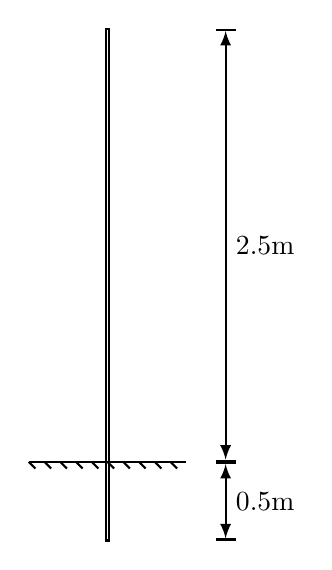
\begin{tikzpicture}[
        >=latex, thick,
    ]
    \draw (-1cm, 0cm) -- (1cm, 0cm);
    \draw[decoration={border,segment length=2mm,amplitude=1.2mm,
                      mirror,angle=45},decorate] (-1cm, 0cm) -- (1cm, 0cm);

    \draw (-0.19mm, -1cm) rectangle (0.19mm, 5.5cm);

    \draw[|<->|] (1.5cm, 0cm) -- (1.5cm, 5.5cm);
    \draw (1.5cm, 2.75cm) node[right] {$2.5\metre$};

    \draw[|<->|] (1.5cm, 0cm) -- (1.5cm, -1cm);
    \draw (1.5cm, -0.5cm) node[right] {$0.5\metre$};

    \end{tikzpicture}
    \caption{Side view of a single pole}
\end{figure}

\begin{figure}[h]
    \centering
    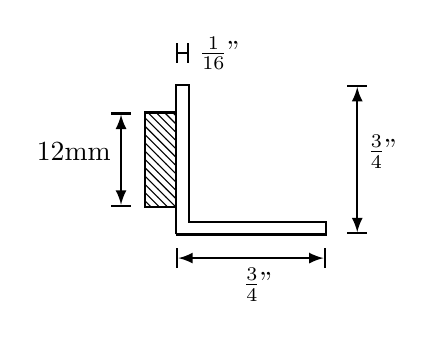
\begin{tikzpicture}[
        >=latex, thick,
    ]
    \draw (0mm, 0mm) -- (0mm, 19mm) -- (1.6mm, 19mm) --
          (1.6mm, 1.6mm) -- (19mm, 1.6mm) --  (19mm, 0mm) -- (0mm, 0mm);

    \draw[pattern=north west lines]
        (0mm, 3.5mm) -- (-4mm, 3.5mm) -- (-4mm, 15.5mm) -- (0mm, 15.5mm);

    \draw[|<->|] (0mm, -3mm) -- (19mm, -3mm);
    \draw (10.5mm, -3mm) node[below]{$\frac{3}{4}"$};

    \draw[|<->|] (23mm, 0mm) -- (23mm, 19mm);
    \draw (23mm, 10.5mm) node[right]{$\frac{3}{4}"$};

    \draw[|-|] (0mm, 23mm) -- (1.6mm, 23mm);
    \draw (1.6mm, 23mm) node[right]{$\frac{1}{16}"$};

    \draw[|<->|] (-7mm, 3.5mm) -- (-7mm, 15.5mm);
    \draw (-7mm, 10.5mm) node[left]{$12\milli\metre$};
    \end{tikzpicture}
    \caption{Top view of a single pole with LED strip}
\end{figure}

%%%%%%%%%%%%%%%%%%%%%%%%%%%%%%%%%%%%%%%%%%%%%%%%%%%%%%%%%%%%%%%%%%%%%%%%%%%
\section{Structural Design Verification}

\begin{figure}[h]
    \centering
    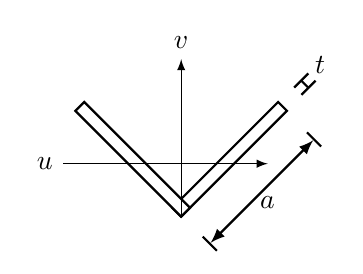
\begin{tikzpicture}[
            >=latex, thick,
    ]
    \draw[rotate=-45,fill=white] (0, 0) rectangle (-1.588mm, 19mm);
    \draw[rotate=45,fill=white] (0, 0) rectangle (1.588mm, 19mm);

    \draw[rotate=45, |<->|] (0, -5mm) -- (19mm, -5mm);
    \draw[rotate=45] (10.5mm, -5mm) node[below] {$a$};

    \draw[rotate=45, |-|] (23mm, 0mm) -- (23mm, 1.588mm);
    \draw[rotate=45] (23mm, 0.8mm) node[above right] {$t$};

    \draw[thin,->] (-15mm, 6.72mm) -- (11mm, 6.72mm);
    \draw (-15mm, 6.72mm) node[left] {$u$};

    \draw[thin,->] (0mm, 0mm) -- (0mm, 20mm);
    \draw (0mm, 20mm) node[above] {$v$};
    \end{tikzpicture}
    \caption{Second Moment of Area for Angle Section}
\end{figure}

\begin{figure}[h]
    \centering
    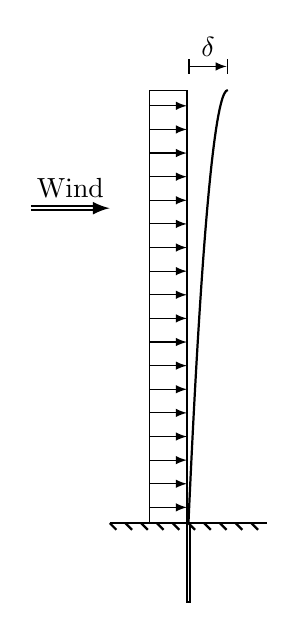
\begin{tikzpicture}[
        >=latex, thick,
    ]
    \draw (-1cm, 0cm) -- (1cm, 0cm);
    \draw[decoration={border,segment length=2mm,amplitude=1.2mm,
                      mirror,angle=45},decorate] (-1cm, 0cm) -- (1cm, 0cm);

    \draw (-0.19mm, -1cm) rectangle (0.19mm, 0cm);
    \draw[thick] (5mm, 5.5cm) parabola (0mm, 0cm);

    \draw[->,double] (-2cm, 4.0cm) -- (-1cm, 4.0cm);
    \draw (-1.5cm, 4.0cm) node[above]{Wind};

    \draw[thin] (-0.5cm, 0) rectangle (-0.19mm, 5.5cm);

    \foreach \y in {0.2, 0.5, ..., 5.5}
        \draw[thin,->] (-0.5cm, \y) -- (-0.19mm, \y);

    \draw[thin,|->|] (0cm, 5.8cm) -- (0.5cm, 5.8cm);
    \draw (0.25cm, 5.8cm) node[above] {$\delta$};

    \end{tikzpicture}
    \caption{Wind loading on pole}
\end{figure}

\section{Electronics Schematic}

\section{Cable layout}
\begin{figure}[h]
    \centering
    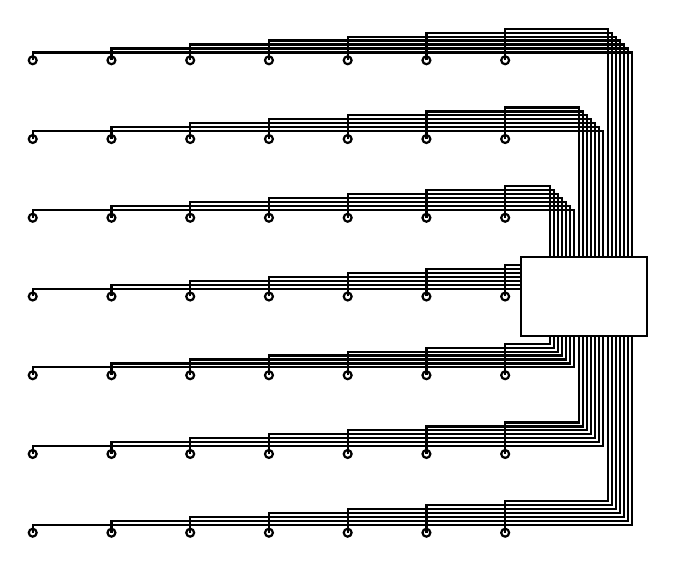
\begin{tikzpicture}[
        >=latex, thick,
    ]

    \foreach \x in {0cm, 1cm, 2cm, 3cm, 4cm, 5cm, 6cm}
        \foreach \y in {-3cm, -2cm, -1cm, 0cm, 1cm, 2cm, 3cm}
            \draw (\x, \y) circle (0.5mm);

    \foreach \x in {0cm, 1cm, 2cm, 3cm, 4cm, 5cm, 6cm}
        \foreach \y in {-3cm, -2cm, -1cm, 0cm, 1cm, 2cm, 3cm}
            \draw (\x, \y) -- (\x, \y + 1mm + \x/20) --
                  ($(6.5cm, \y) + (0, \x/20 + 1mm) - (\x/20, 0) + abs(\y)*(0.13mm, 0)$)
                  -- ++(0, -\y);

    \draw[fill=white] (6.2cm, -0.5cm) rectangle (7.8cm, 0.5cm);


    \end{tikzpicture}
    \caption{Power/control cable routing}
\end{figure}


\section{Prototype Pole}

\end{appendices}

\end{document}

